\section{Methodology}

The methodology of this lab exercise follows the usual process for machine learning problems/researches
\[
  \text{data} \to \text{preprocessing} \to \text{modeling} \to \text{evaluation}
\]

The preprocessing section mainly consists of splitting the dataset into training and testing data, checking the validity of data, as well as many others. The Convolutional Neural Network, like other neural networks, can be customized especially in the number of convolutional layers, different pooling methods, different kernels, etc. Unlike previous models, there really isn't much customization that could be done to them other than the hyperparameters to alter slightly how it works. But when it comes to CNNs, there's a lot more room for varying techniques. 

Later in experimentation, we will see how customizing the CNN can affect performance for detecting these hair types. For evaluation, the accuracy metric is used to measure the model's performance. 

\subsection{Data Acquisition and Preparation}

\subsubsection{Loading of Images}

A folder named \texttt{hair\_types} was manually imported in the repository containing 1000 images. Inside that folder has subdirectories for each hair type. Python Imaging Library (PIL) library was used to create a custom function of validating the images that was imported. It ensures that none of these images are corrupted and adhere to specific formats, such as PNG, JPG, and BMP. We excluded files that are not accepted by Tensorflow and does not match the specific formats, such as .WebP. After loading these images, 14 images were deleted and one image with a file type of .gif was also detected, but we didn't remove it because it is still valid for this experiment. This step is important to minimize potential issues during model training.

\subsubsection{Image Categorization}

This step involves segrating the images into three groups based on hair type labels found in their file paths. This will help in the structured training of the model by defining the classes of each images.

\subsubsection{Manual Inspection}

To ensure the integiry of our dataset, we manually inspected each image via the file explorer. During the inspection, we identified irrelevant image of a microphone logo found in the subdirectory folder of \texttt{Straight\_Hair}. Removing this image was crucial to prevent the model from leaning incorrect and unnecessary information.

\subsubsection{Image Display}

Using matplotlib, we displayed a sample from each category. This step is important to ensure the integrity and appropriateness of the labels and the image themselves.

\subsection{Preprocessing}

\subsubsection{Data Augmentation}

Initaially, we tried applying several data augmentation technicques, such as random horizontal and vertical flips, random rotations, and random zooms. However, we didn't apply data augmentation in the final model, which will be discussed on the Experiments section.

\subsubsection{Splitting Dataset}

To ensure generalizability of this model, we utilized Tensorflow's \texttt{image\_dataset\_from\_directory} method to split the image data into training and validation datasets. 20 \% of the data was allocated for validation. Additionally, we resize all images to a uniform \(256 \times 256\) pixels for consistency and batch them in sizes of 64. Splitting the data this way helps prevent overfitting by ensuring that the model does not memorize the training data and allows us to fine-tune the model parameters based on the performance metrics gathered from validation set.

\subsubsection{Sobel Edge Detection}

A custom preprocessing function was created to detect Sobel edges in the images. This technique highlights the edges within each image. This technique will be applied for both training sets and validation sets to ensure consistency in how images are presented to the model.

We generated 9 samples from the dataset to display sobel edges applied images.

\begin{figure}[H]
  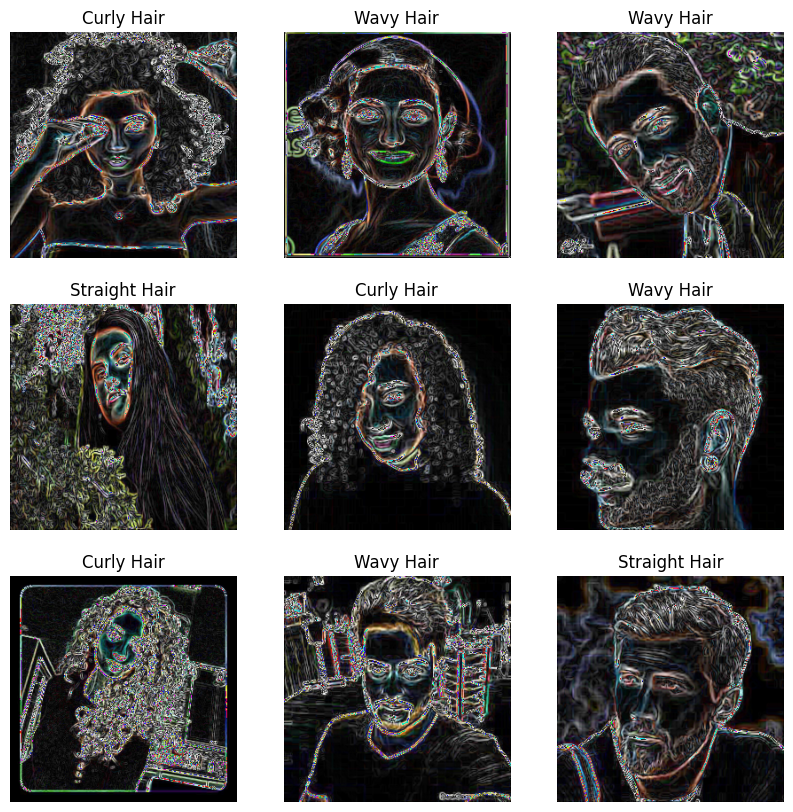
\includegraphics[width=\linewidth]{figures/sobel_edge_images.png}
  \caption{Hair Types Example with Sobel Edge}
  \label{fig:sobel_edge_hairtypes}
\end{figure}

\subsection{Modeling}

\subsubsection{Convolutional Neural Network Architecture}

In this step, we constructed a convolutional neural network (CNN) model using the Keras library's `Sequential` API. The network begins with a rescaling layer that normalizes the pixel values of the images from a range of 0 to 255 to a range of 0 to 1, enhancing the training efficiency. 

The architecture of our convolutional neural network (CNN) begins with the `Sequential` model framework from Keras, which allows layers to be added sequentially. 

1. Input Layer: This layer specifies the shape of the input data, which is 256x256, and adds three color channgels (RGB), making it \(256, 256, 3\).

2. Rescaling Layer: After the input layer, a \texttt{Rescaling} layer npormalizes the pixel values of the images from a range of 0 to 255 to a range of 0 to 1. This is important because it helps the model converge faster during the training stage.

3. First Convolution Layer: This layer uses 16 filters with a kernel size of 16 and a stride of 2. We also did not added padding in the input (\texttt{valid padding}). The dilation rate is set to 1, which keeps the kernel compact.

4. Activation Function: Every after convolution layer, a Rectified Linear Unit (ReLU) activation function is applied. This is used to introduce non-linearity to the model and solves the vanishing gradients issue.

5. Batch Normalization: This normalization technique is applied to help standardizing the data by normalizing the activation of the convolution layer.

6. Pooling Layer: After that, \texttt{MaxPooling2D} layer is applied to reduce the spatial dimentions of the output. It summarizes the features in a 2x2 window with the maximum value.

7. Dropout Layer: A dropout layer is introduced with a rate of 0.25 to help prevent overfitting by randomly setting a fraction of input unit to 0 during training.

8. Other Convolution Layers: The process above is repeated three more times with different filter and kernel sizes. The filters increase while the kernel size decrease as the process continue. For the last two convolution layers, max pooling and dropout were excluded.

9. Global Average Pooling: After the last convolutional layers, a \texttt{GlobalAveragePooling2D} layer is applied, which calculates the average value of each feature map and outputs a tensor that is smaller in size. This can help reduce the dimensionality of the feature maps and prevent overfitting. 

10. Flattening: After that, a \texttt{Flatten} layer then converts these features into a single vector. This helps maintain all the information from the feature maps and connect the convolutional layers to the fully connected layers.

10. Dense and Output Layers: The feature vector coming from the Flattening layer is fed into a dense layer of 32 neurons, followed by a dropout layer with a rate of 0.5, and then an activation function of ReLU. The final output layer will consists of 3 neurons (one for each hair type) with a \texttt{softmax} activation function.

\subsubsection{Training the Model}

The model was compiled with the Adam optimizer, using a learning rate of \texttt{1e-4} and categorical cross-entropy loss function because the dataset consist of multiple classes. The training was conducted over 50 epochs, using both training and validation datasets.

\begin{figure}[H]
  \centering
  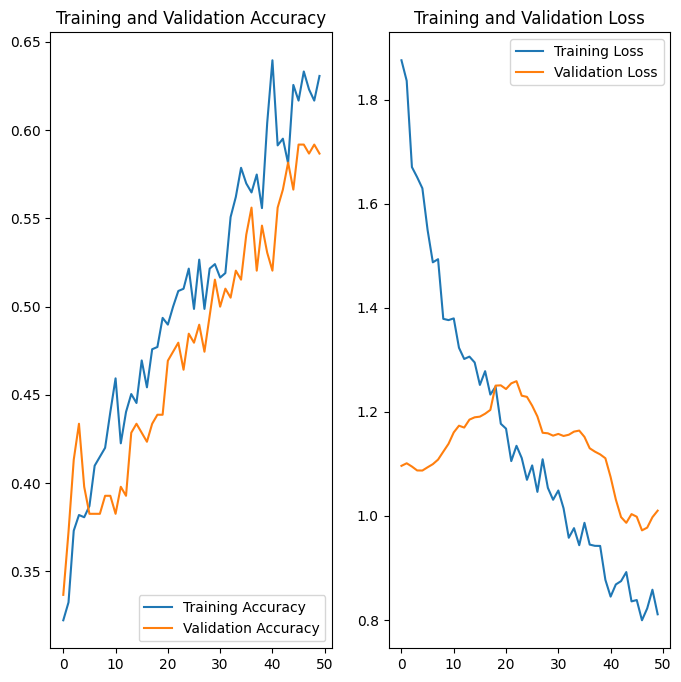
\includegraphics[width=0.8\linewidth]{figures/training_validation_results.png}
  \caption{Training and Validation Results}
  \label{fig:results}
\end{figure}

\subsection{Evaluation}

To evaluate the performance of the convolutional neural network, we utilized different techniques that visually and quantitavely assess its effectiveness:

1. Accuracy and Loss Plots: We generated line plots to compare the training and valiation accuracy, as well as the training and validation loss over the epochs. These plots are important for us to understand the model's learning progress and see if it is overfitting or not.

2. Confusion Matrix: We created a confusion matrix from \texttt{sklearn.metrics} to visually inspect the performance of the model across different classes. It can also help us identify misclassifications in the model.

3. Classification Metrics Report: We utilized the \texttt{classification\_report} from \texttt{sklearn.metrics} to see the results of the precision, recall, and F1-score for each class. 

4. Image Prediction: Finally, to demonstrate the effectiveness of the model in predicting the hair type of the image, we used the \texttt{predict} method to see the percentage of each classes based on a single image.
